\documentclass{beamer}
\usetheme{metropolis}

\usepackage{microtype}
\usepackage{changepage}
\usepackage{graphicx}
\usepackage{tikz}
\usetikzlibrary{calc}  % Add calc library for better TikZ control
\usepackage{subcaption} % For side-by-side figures with captions


\theoremstyle{definition}
\newtheorem{noitalicstheorem}{Theorem}

\DeclareMathOperator{\GL}{GL}
\DeclareMathOperator{\M}{M}

\newcommand{\C}{k}
\renewcommand{\O}{\mathcal{O}}
\newcommand{\Q}{\mathbb{Q}}
\newcommand{\Z}{\mathbb{Z}}
\newcommand{\p}{\mathfrak{p}}

\usetheme{metropolis}
\definecolor{mynavy}{RGB}{35, 55, 59}
\definecolor{myorange}{RGB}{235, 129, 27}
\definecolor{myteal}{RGB}{92, 188, 172}
\definecolor{mygreen}{RGB}{11, 176, 161}
\definecolor{myblue}{RGB}{130, 158, 117}
\metroset{block=fill}

\theoremstyle{definition}
\newtheorem{nullstellensatz}{The Nullstellensatz (Moral)}
\newtheorem{proposition}{Proposition}
%\newtheorem{theorem}{Theorem}

\title{Toric Varieties}
\subtitle{Bridges in Algebra and Geometry}
\author{Declan Fletcher}
\date{October 2024}

\begin{document}
\begin{frame}
\titlepage
\end{frame}

\begin{frame}
\frametitle{Two bridges}
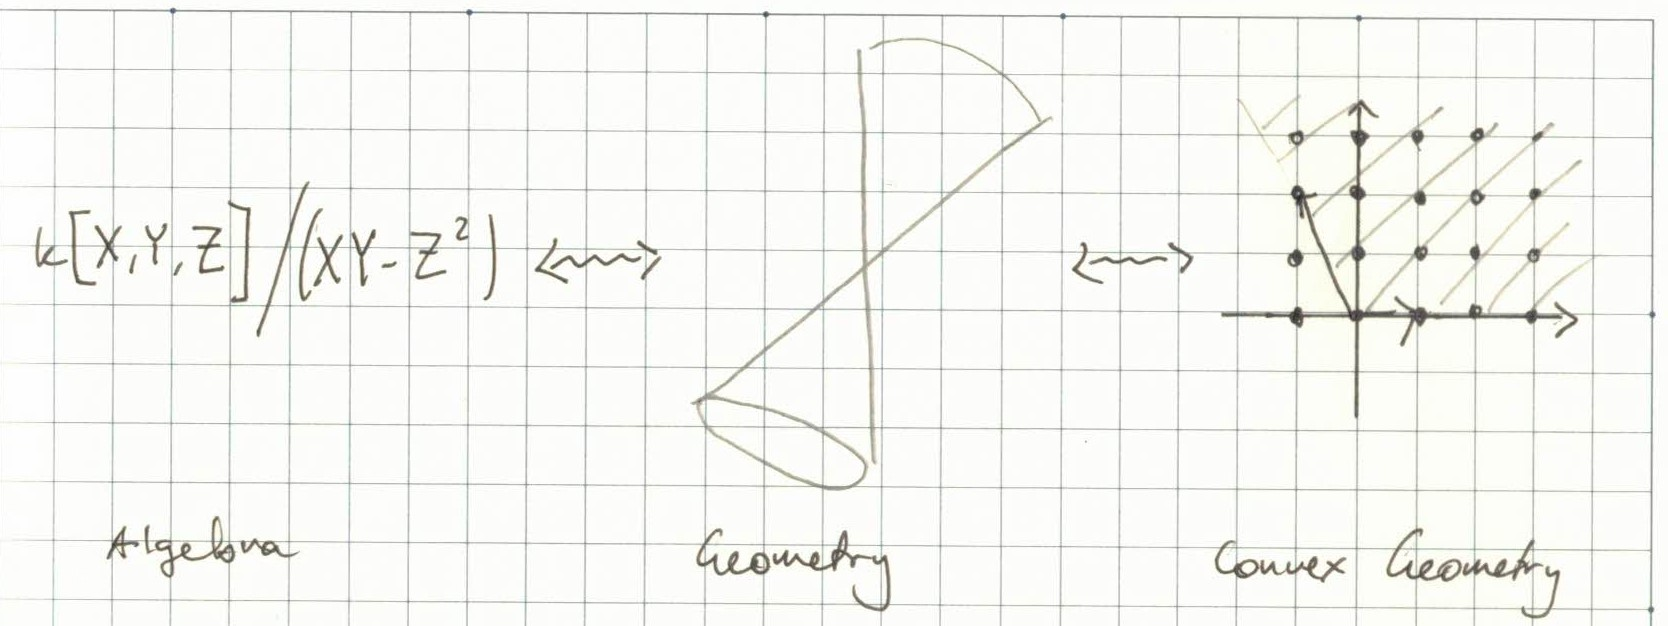
\includegraphics[width=\textwidth]{ring_variety_cone}
\end{frame}

\begin{frame}
\frametitle{Overview}
\centering
\begin{enumerate}
\item Affine varieties
\item Polynomial maps
\item The Nullstellensatz
\item Irreducibility and prime ideals
\item Singularities
\item Convex cones
\item Toric varieties
\item Faces and open subsets
\item Singularities of toric varieties
\end{enumerate}
\end{frame}

\begin{frame}
\frametitle{Affine varieties}
Let $k$ be a field.
The set of $n$-tuples of elements of $k$ is called affine space, $\mathbb{A}^n$.
Given a polynomial $f$ in $k[X_1, \ldots, X_n]$, we can consider its zero set
$$\mathbf{V}(f) := \{(a_1, \ldots, a_n) \in \mathbb{A}^n : f(a_1, \ldots, a_n) = 0\}.$$
\centerline{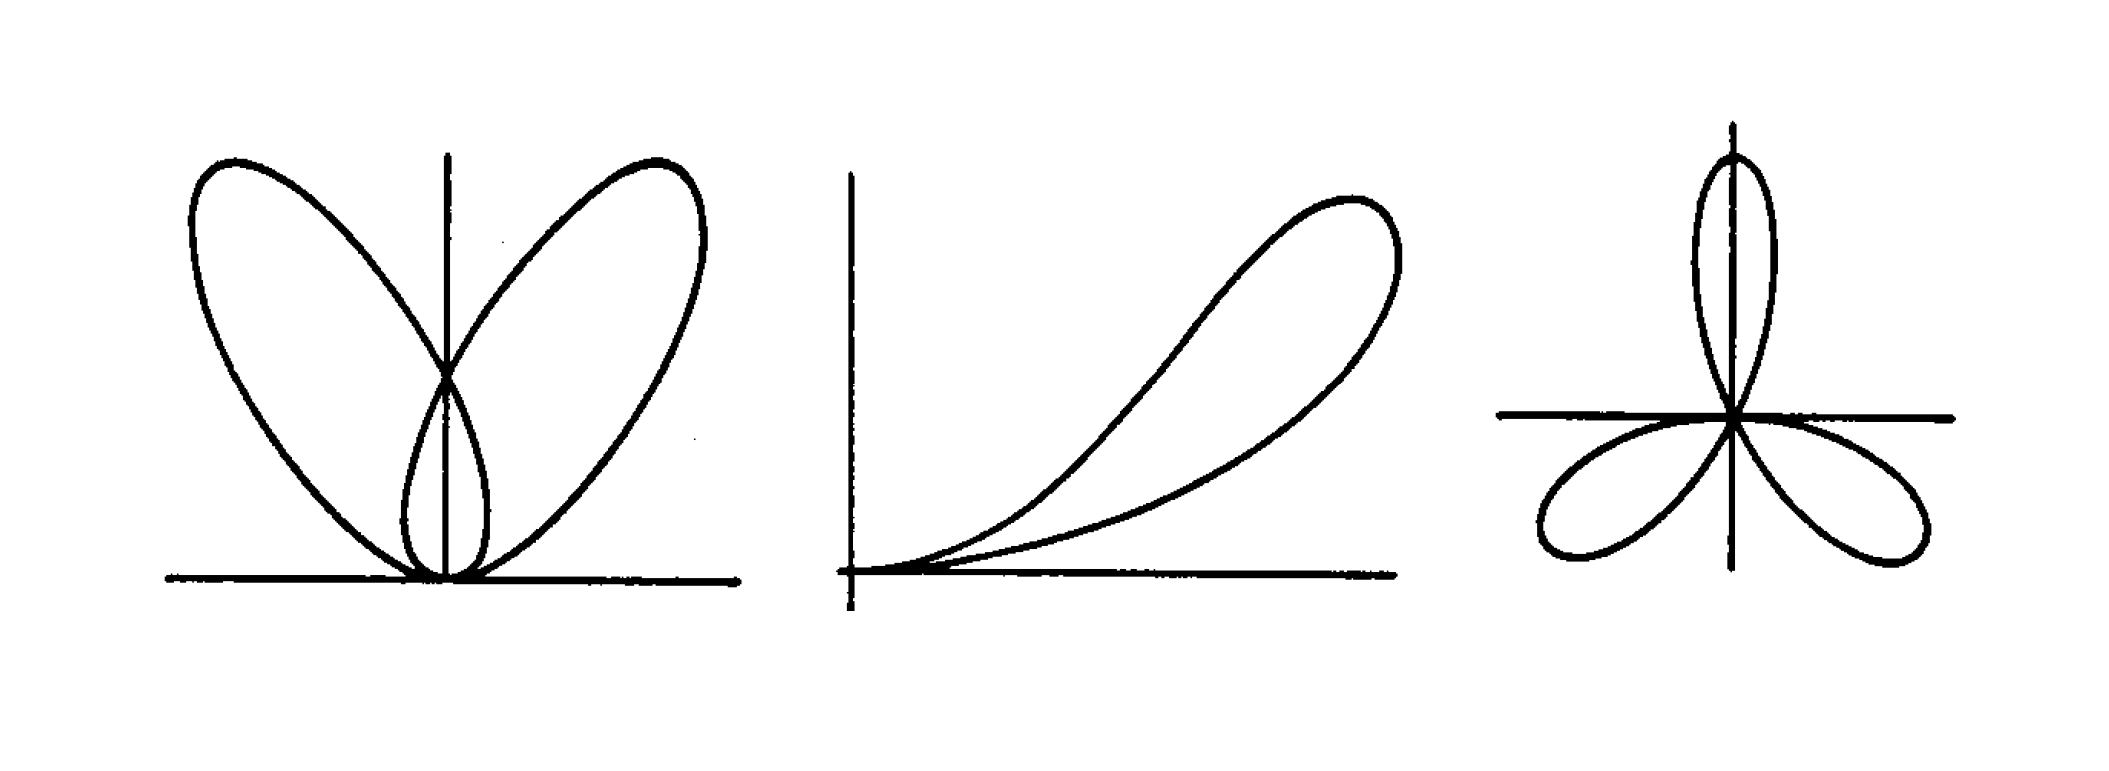
\includegraphics[width=0.6\textwidth]{milne_three_curves}}
We can also consider spaces cut out by sets of polynomials $I \subseteq k[X_1,\ldots,X_n]$: 
$$\mathbf{V}(I):=\{(a_1, \ldots, a_n) \in \mathbb{A}^n : f(a_1, \ldots, a_n) = 0 \text{ for all } f \in I\}.$$
These spaces are called \alert{affine varieties}.
\end{frame}

\begin{frame}
\frametitle{Varieties throughout mathematics}
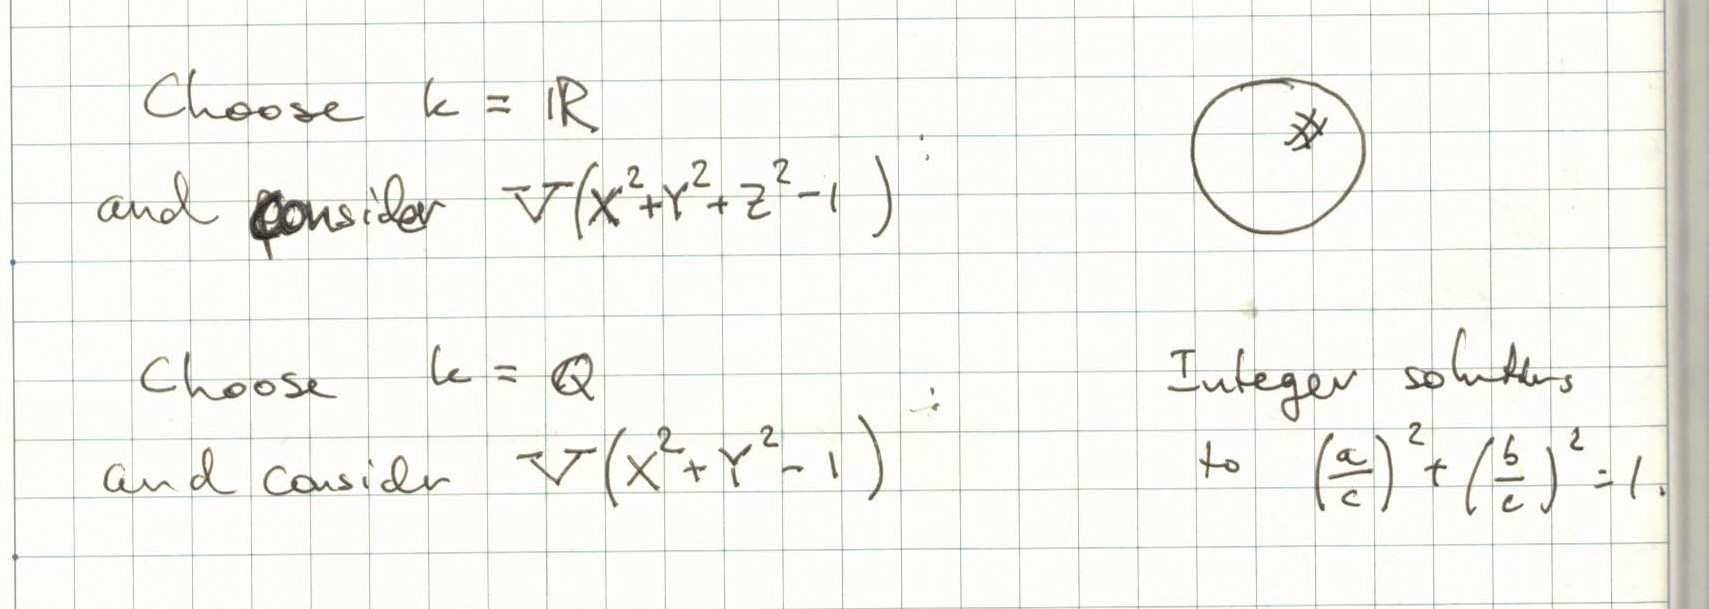
\includegraphics[width=\textwidth]{sphere_and_pythag_triples}
\end{frame}

\begin{frame}
\frametitle{The Zariski topology}
Affine space is endowed with the \alert{Zariski topology}.

This is the topology defined by declaring $S \subseteq \mathbb{A}^n$ closed if
$$S = \mathbf{V}(I)$$
for some $I \subseteq k[X_1, \ldots, X_n]$.

The Zariski topology on a variety $V$ is the induced topology from $\mathbb{A}^n$.

\centerline{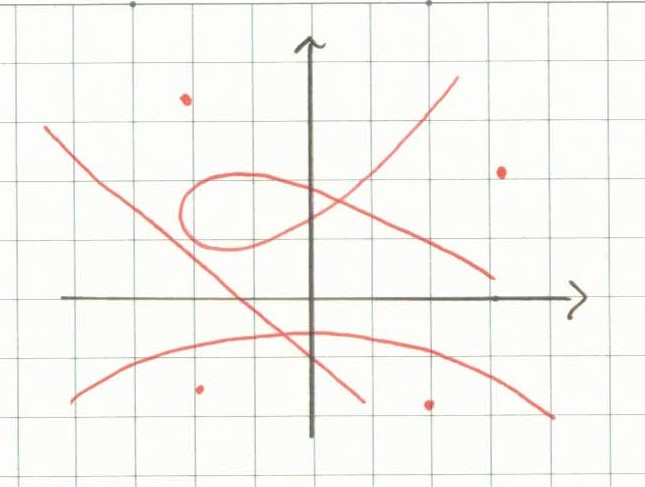
\includegraphics[width=0.4\textwidth]{zariski_open}}
\end{frame}

\begin{frame}
\frametitle{Polynomial functions}
% Define polynomial function
We say a function $V \to k$ is \alert{polynomial} if it is the restriction of a polynomial function $\mathbb{A}^n \to k$.

Problem: different polynomials give the same function.
For example, on the circle $V = \mathbf{V}(X^2+Y^2-1)$, the polynomials
$$2 X Y^2, \qquad 2 X Y^2 - 2X (X^2+Y^2-1)$$
define the same function.

Solution: consider functions in the quotient
$$k[V] := k[X_1, \ldots, X_n] / \mathbf{I}(V),$$
where
$$\mathbf{I}(V) := \{\text{polynomials vanishing on $V$}\}.$$
We call $k[V]$ the \alert{coordinate ring} of $V$, and $\mathbf{I}(V)$ the \alert{ideal} of $V$.

% Define the ideal $\mathbf{I}$ and the coordinate ring. 
\end{frame}

\begin{frame}
\frametitle{Polynomial maps}
%Define polynomial map $V \to W$.
A map $\varphi : V \subseteq \mathbb{A}^n \to W \subseteq \mathbb{A}^m$ is called \alert{polynomial} if its components are polynomial functions on $V$, i.e., if
$$\varphi = (\varphi_1, \ldots, \varphi_m)$$
for some $\varphi_i \in k[V]$.

%Explain how these are $k$-algebra homomorphism $k[W] \to k[V]$.

%Isomorphic algebraic sets if and only if isomorphic $k$-algebras.

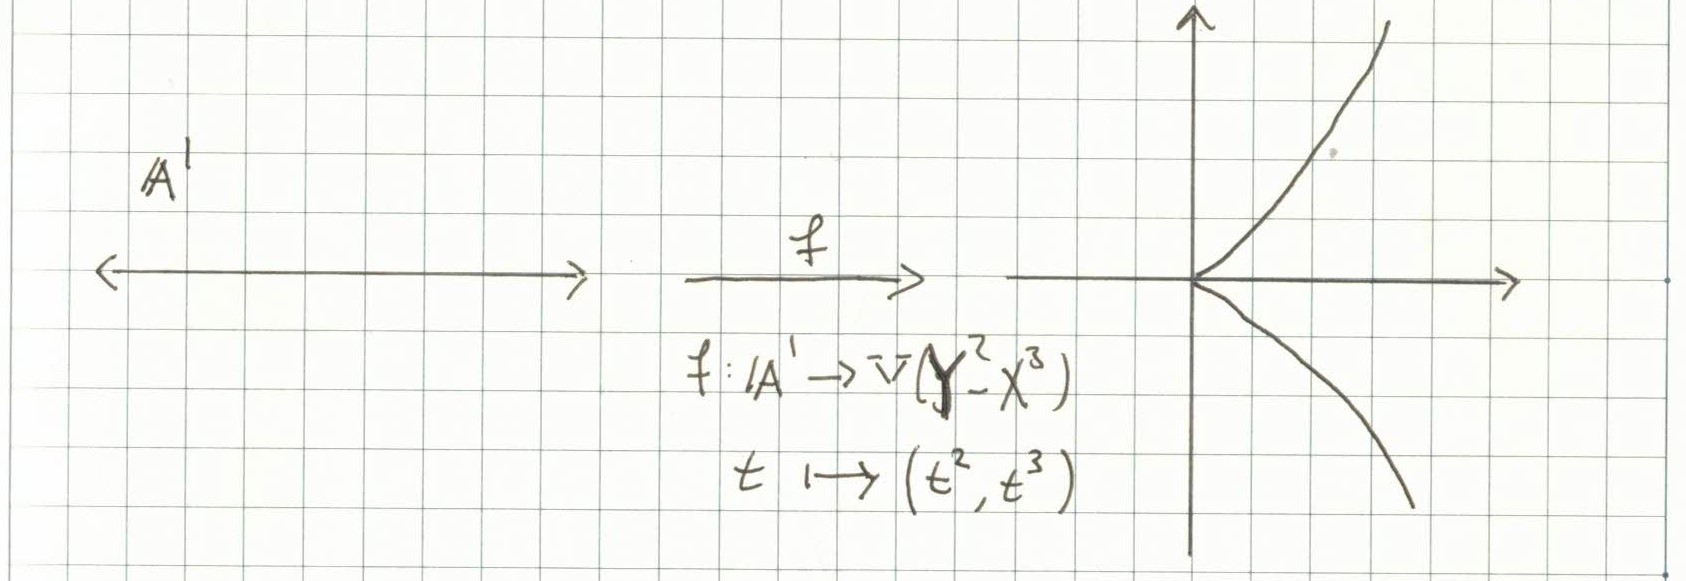
\includegraphics[width=\textwidth]{polynomial_map}

We say $\varphi$ is an isomorphism if it is bijective with polynomial inverse.
\end{frame}

\begin{frame}
\frametitle{The Nullstellensatz}
We have maps
$$\{ \text{varieties in } \mathbb{A}^n \} \underset{\mathbf{V}}{\overset{\mathbf{I}}{\rightleftarrows}}  \{\text{ideals in } k[X_1, \ldots, X_n] \}.$$

\begin{nullstellensatz}
Let $k$ be \alert{algebraic closed}.
There is a bijection
$$\{ \text{varieties in } \mathbb{A}^n \} \leftrightarrow \{\text{\alert{radical} ideals in } k[X_1, \ldots, X_n] \}.$$
\end{nullstellensatz}

An ideal $I$ is called radical if whenever $f^n \in I$ for some $n \in \mathbb{Z}_{> 0}$, we have $f \in I$.
These are ideals containing all their square roots, cube roots, etc.

Henceforth, we assume $k$ is algebraically closed.
\end{frame}

\begin{frame}
\frametitle{Maps and homomorphisms}
A polynomial map $\varphi : V \to W$ gives us a rule for turning polynomial functions on $W$ into polynomial functions on $V$.
Specifically, it gives a ring \alert{homomorphism}
$$\varphi^* : k[W] \to k[V], \qquad f \mapsto \varphi^* f := f \circ \varphi.$$
\centerline{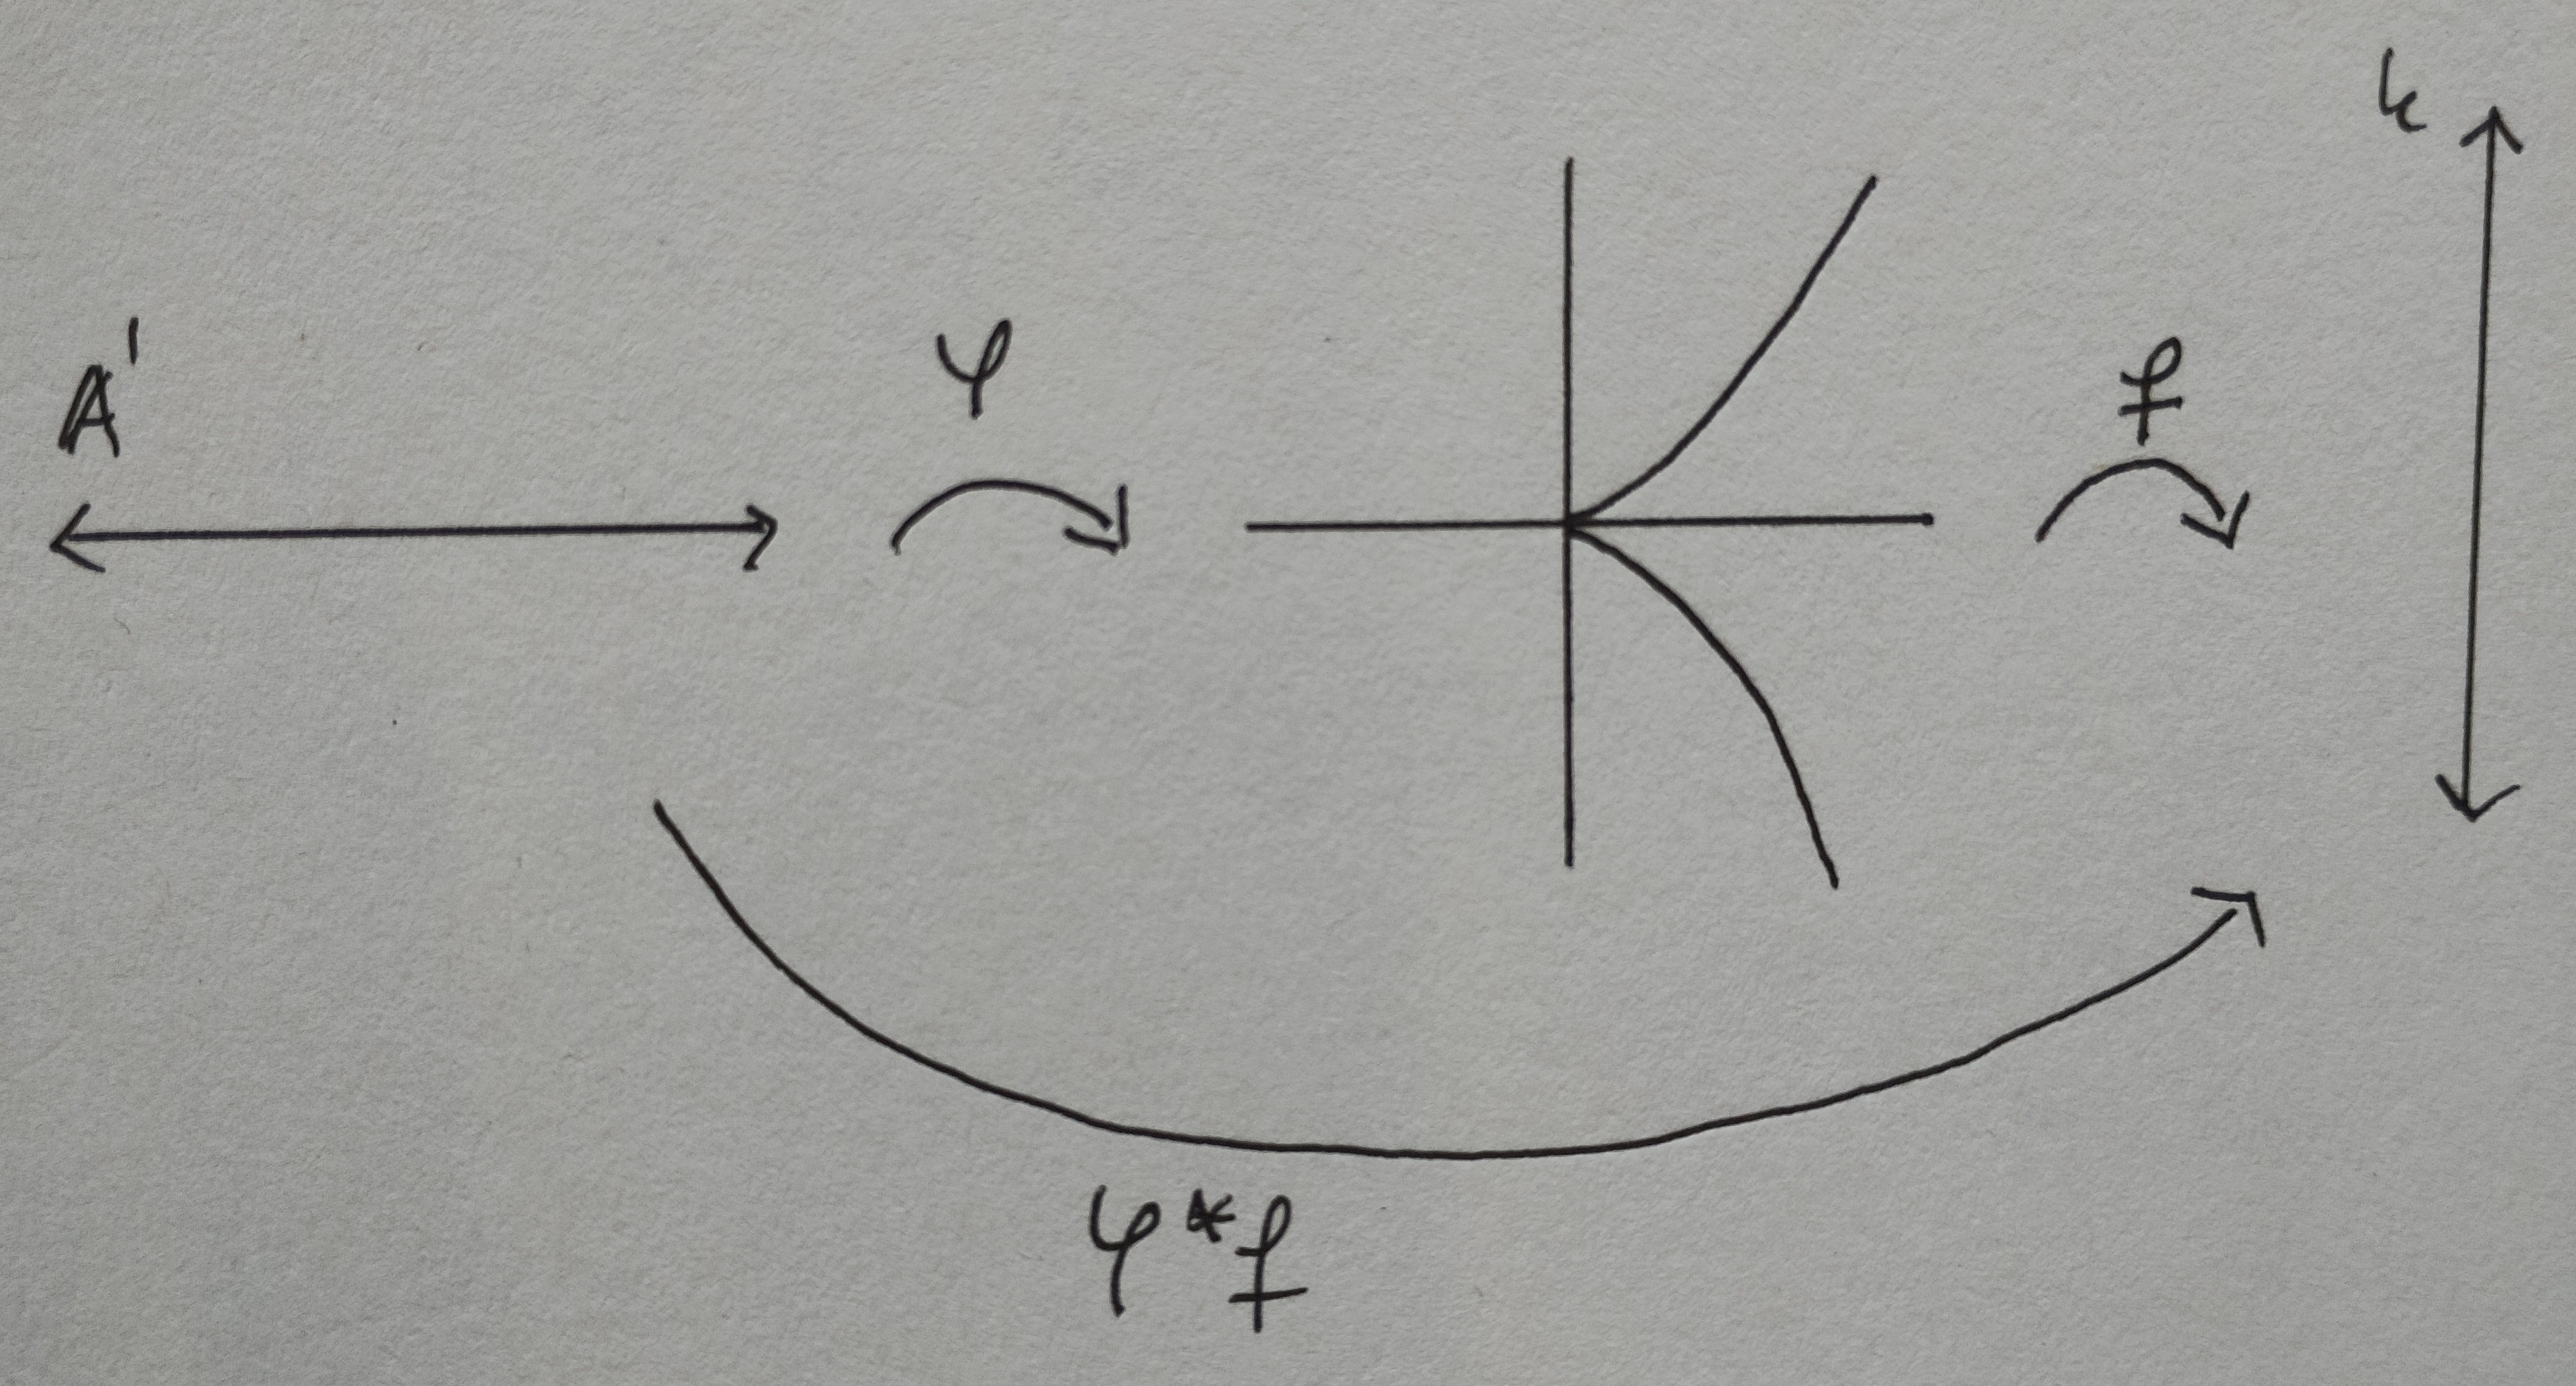
\includegraphics[width=0.5\textwidth]{pullback}}
The map $\varphi \mapsto \varphi^*$ is in fact a bijection
\begin{align*}
\left\{
\begin{array}{c}
	\text{poly. maps } V \to W \\
	%V \to W
\end{array}
\right\} \longleftrightarrow 
\left\{
\begin{array}{c}
	\text{ring homs } k[W] \to k[V] \\
	%k[W] \to k[V]
\end{array}
\right\}.
\end{align*}
Moreover, $\varphi$ is an isomorphism if and only if $\varphi^*$ is.
Then $V$ and $W$ are isomorphic if and only if $k[V]$ and $k[W]$ are.
\end{frame}

\begin{frame}
\frametitle{Irreducibility and prime ideals}
We say a variety is \alert{irreducible} if it is not the union of two proper closed subsets.
\centerline{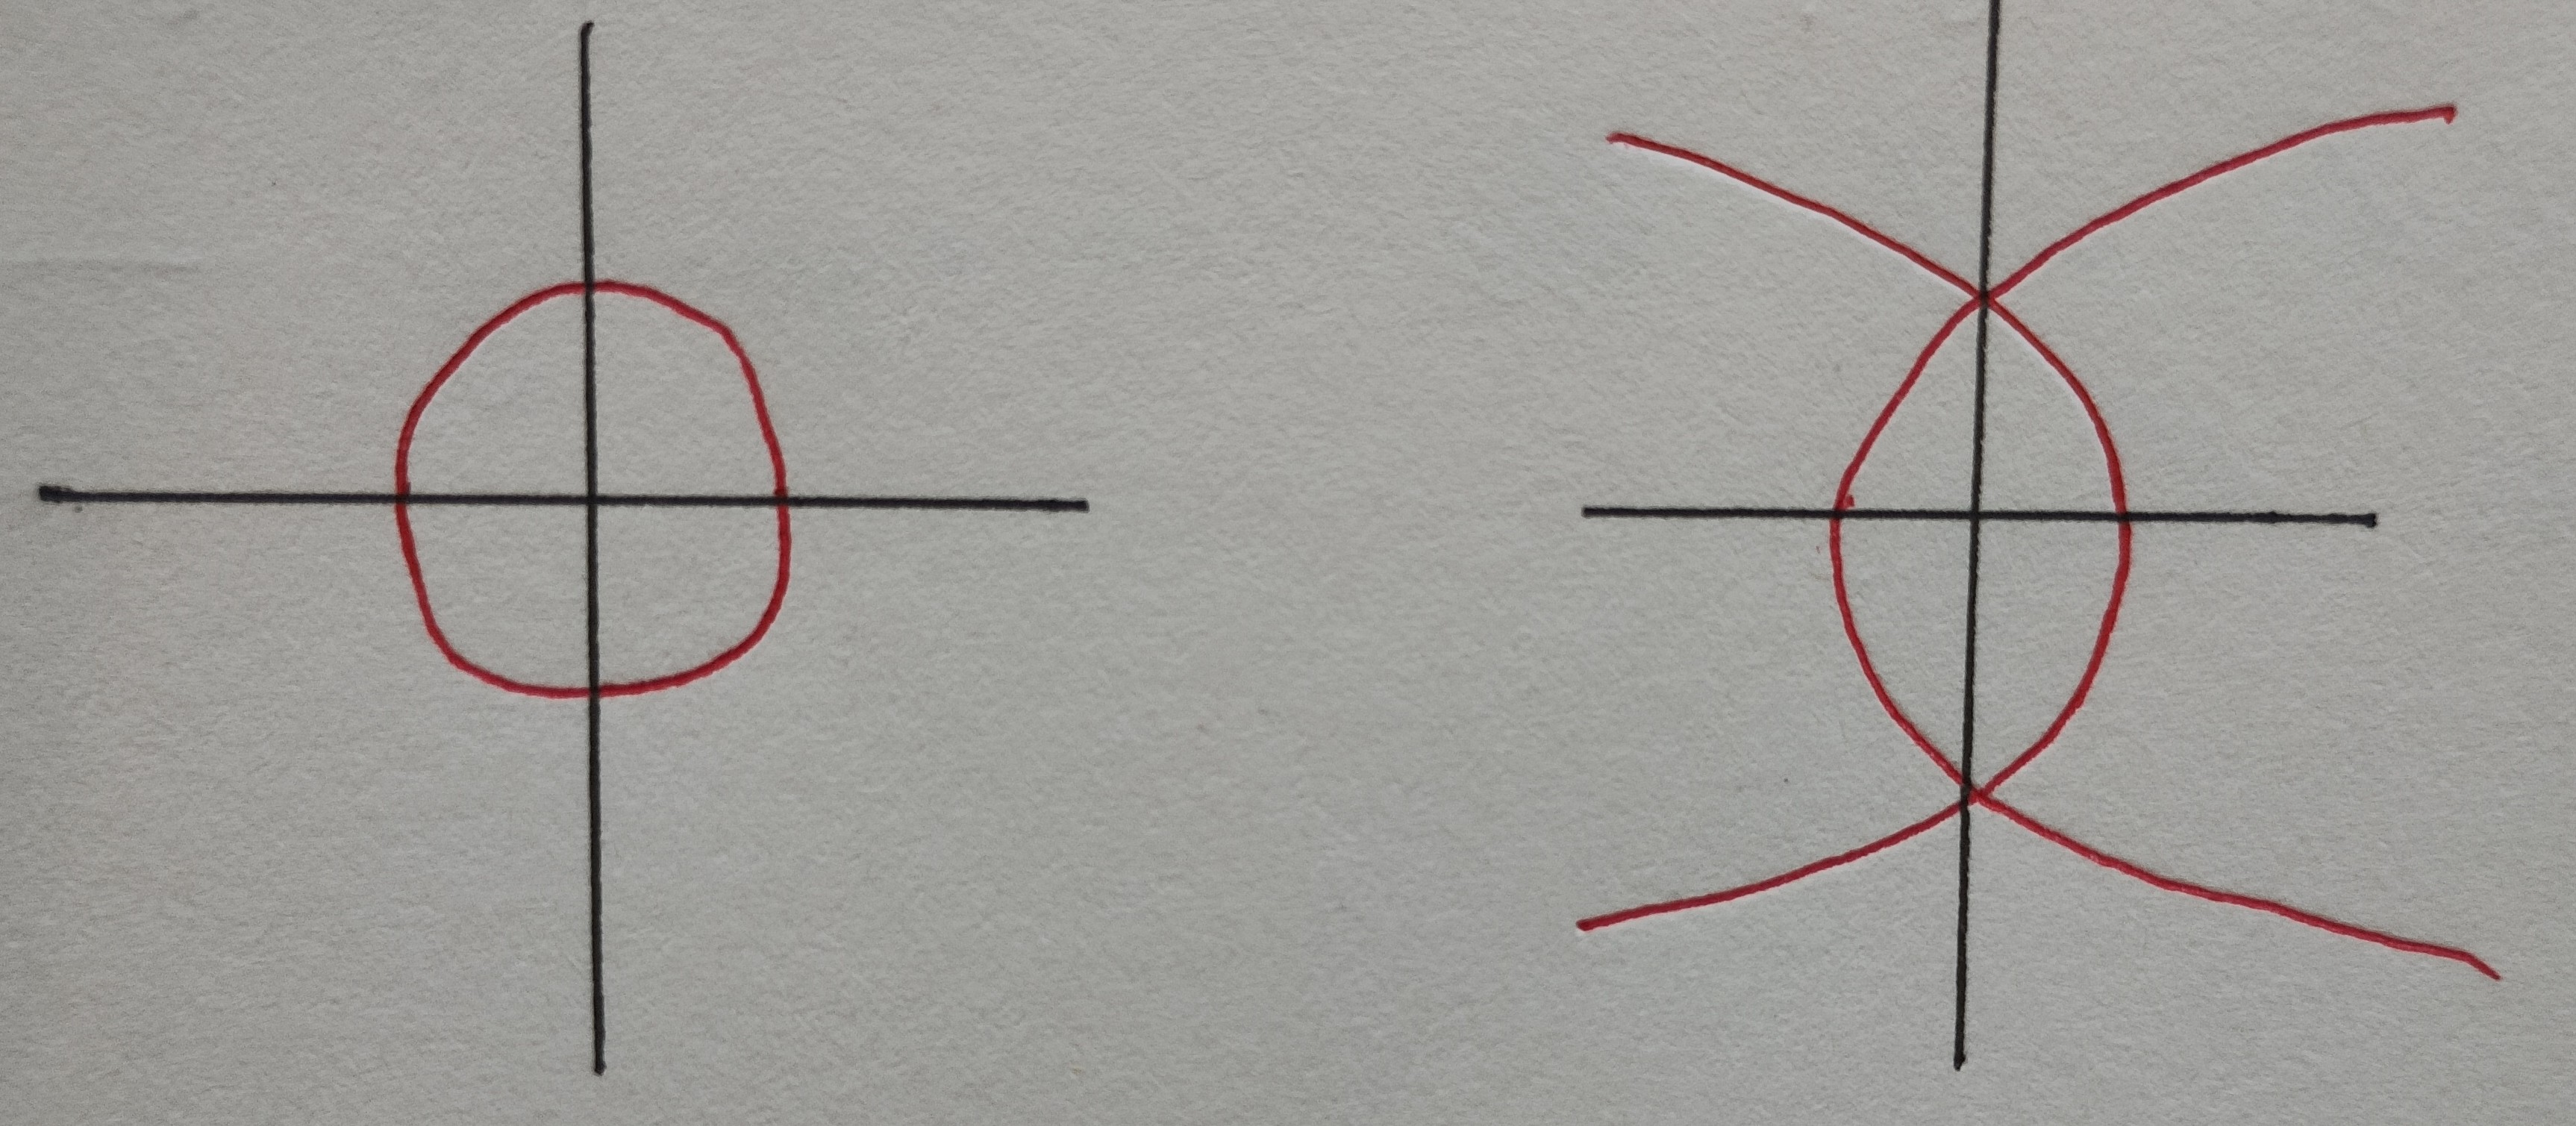
\includegraphics[width=0.6\textwidth]{irreducibility}}
The ideal $\mathbf{I}(V)$ is \alert{prime} if and only if $k[V] = k[X_1, \ldots, X_n]/\mathbf{I}(V)$ has no zero divisors.

\begin{proposition}
The variety $V$ is irreducible if and only if the ideal $\mathbf{I}(V)$ is prime.
\end{proposition}
\end{frame}

\begin{frame}
\frametitle{Tangent spaces and dimension}
Tangent spaces are an important tool for studying smooth surfaces in differential geometry.
There is an analog for varieties.

We define tangent spaces for the hypersurface $V = \mathbf{V}(f)$.
Let $P = (a_1, \ldots, a_n)$ be a point in $V$.
The first-order part of $f$ at $P$ is
$$f_P^{(1)} := \sum_{i=1}^n \frac{\partial f}{\partial X_i}(P) (X_i-a_i).$$
The \alert{tangent space} of $V$ at $P$ is
$$T_P V:= \mathbf{V}(f_P^{(1)}).$$

The \alert{dimension} of $V$ is 
$$\dim(V) := \min_{P \in V} \dim(T_PV).$$
\end{frame}

\begin{frame}
\frametitle{Singular and non-singular points}
We say a point $P$ is \alert{singular} if 
$$\dim(T_PV) > \dim(V),$$
and non-singular otherwise.

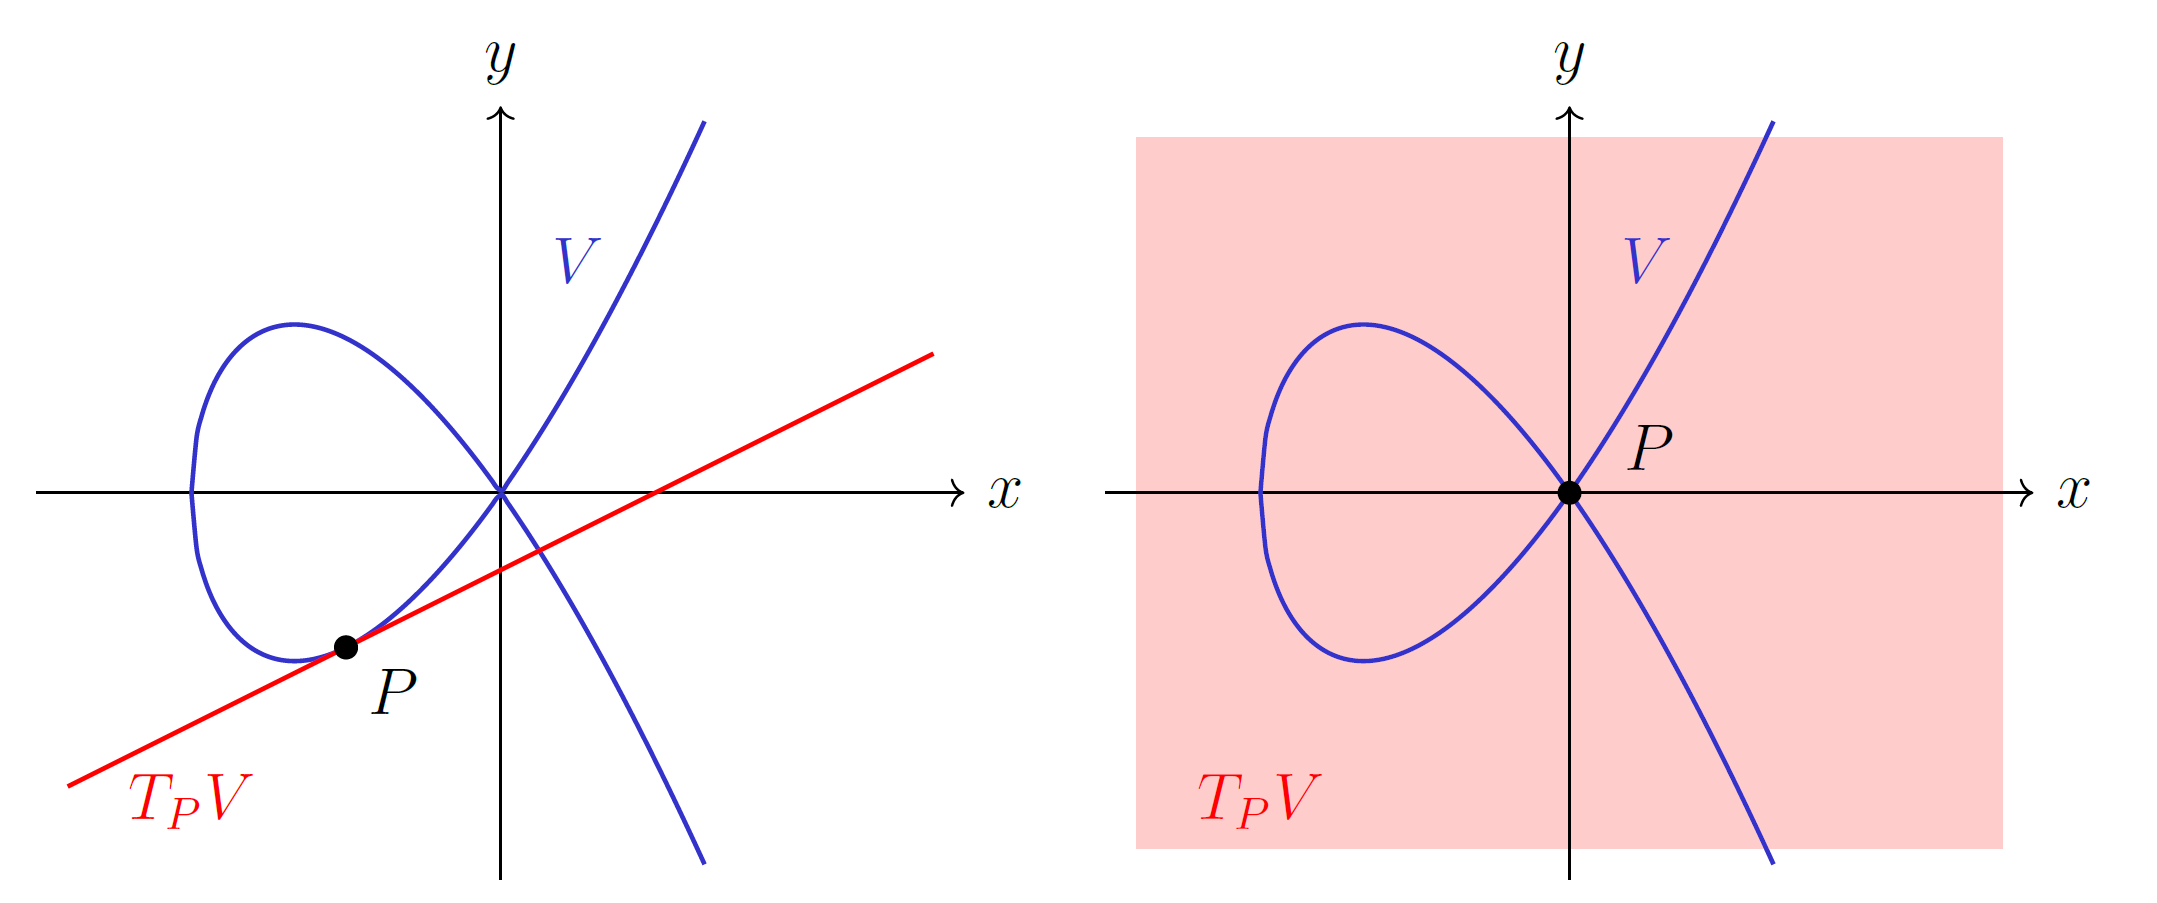
\includegraphics[width=\textwidth]{tangent_spaces}

\end{frame}

\begin{frame}
\frametitle{Convex cones}
A \alert{polyhedral cone} in the vector space $\mathbb{R}^n$ is a set of the form
$$\sigma = \mathrm{span}_{\mathbb{R}_{\ge 0}}\{v_1, \ldots, v_r\},$$
for some vectors $v_1, \ldots, v_r$ in $\mathbb{Z}^n$.

The \alert{dual cone} to a polyhedral cone $\sigma$ is
$$\sigma^\vee := \{u \in (\mathbb{R}^n)^* : u(v) \ge 0 \text{ for all } v \in \sigma\}.$$

\centerline{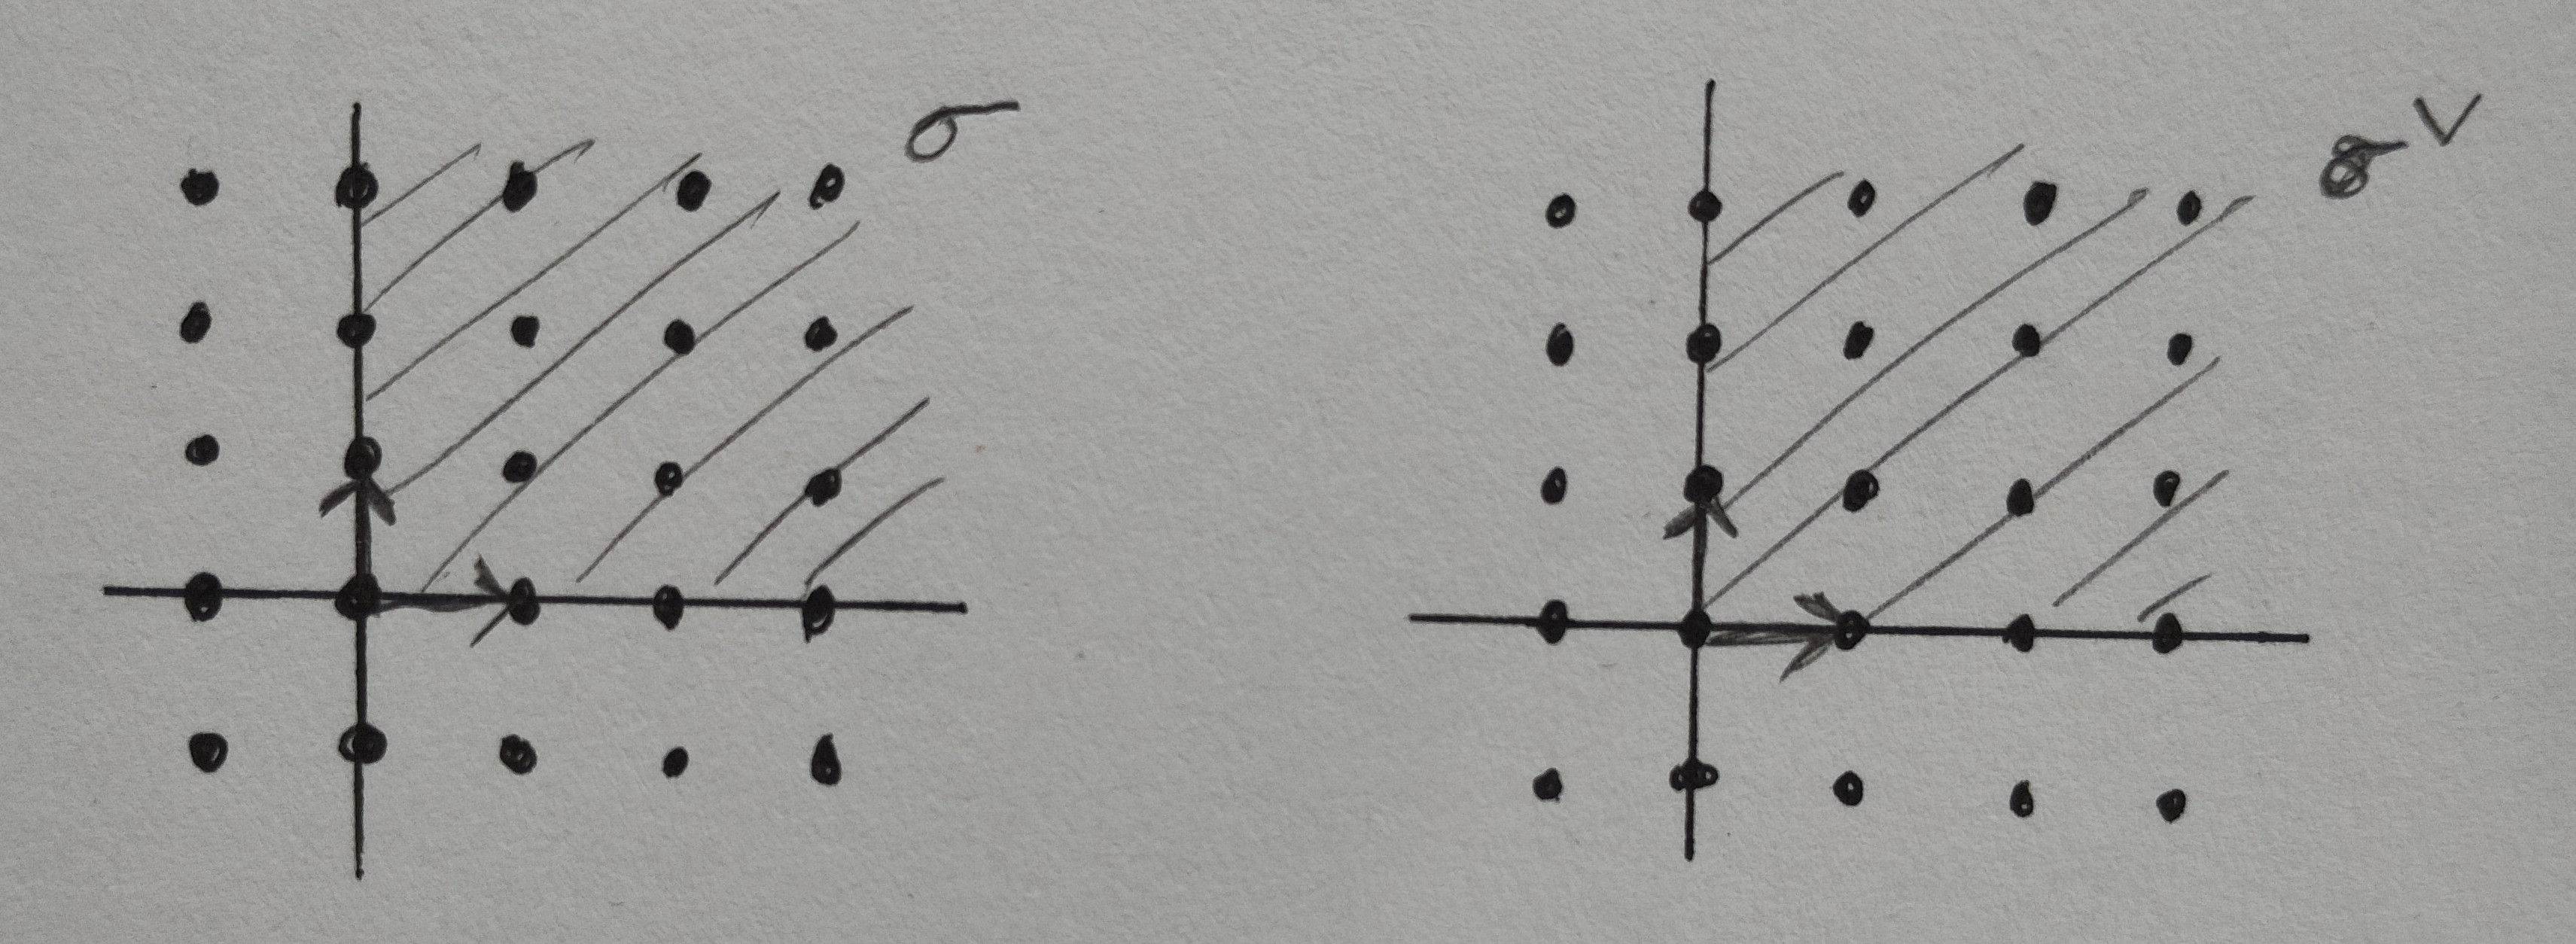
\includegraphics[width=0.65\textwidth]{basic_cone_and_dual}}
\end{frame}

\begin{frame}
\frametitle{Cones and their duals}
A trivial (but important) example:
if $\sigma = \{0\}$, then $\sigma^\vee = (\mathbb{R}^n)^*$.

For a non-trivial example, consider
$$\sigma = \mathrm{span}_{\mathbb{R}_{\ge 0}}\{e_1, -e_1 + 2 e_2\}.$$
Then,
$$\sigma^\vee = \mathrm{span}_{\mathbb{R}_{\ge 0}}\{2 e_1 + e_2, e_2\}.$$
\centerline{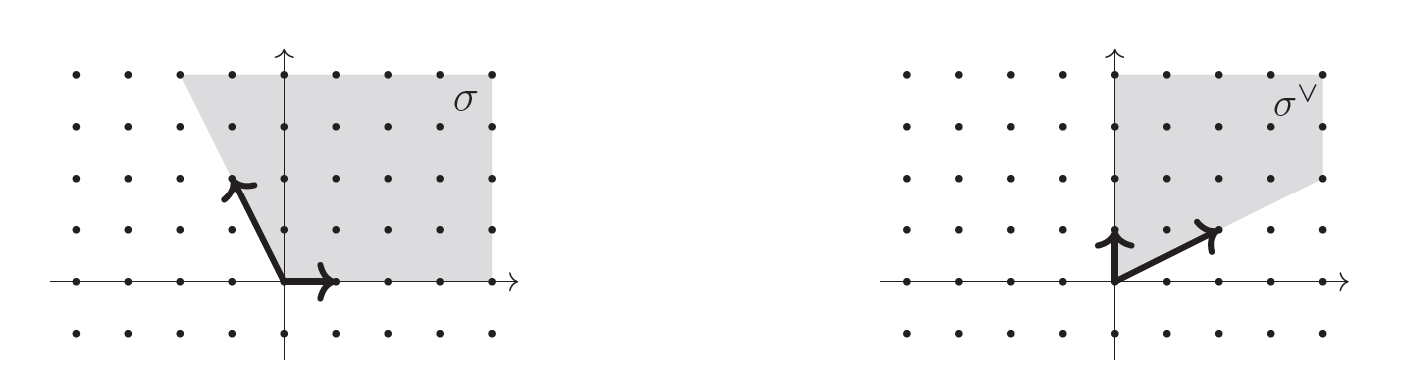
\includegraphics[width=\textwidth]{cone_and_dual}}
\end{frame}

\begin{frame}
\frametitle{Toric varieties, the intuition}
Given a cone and its dual, we place a monomal $X^i Y^j$ on the integer points $(i, j)$ in the dual space:

\centerline{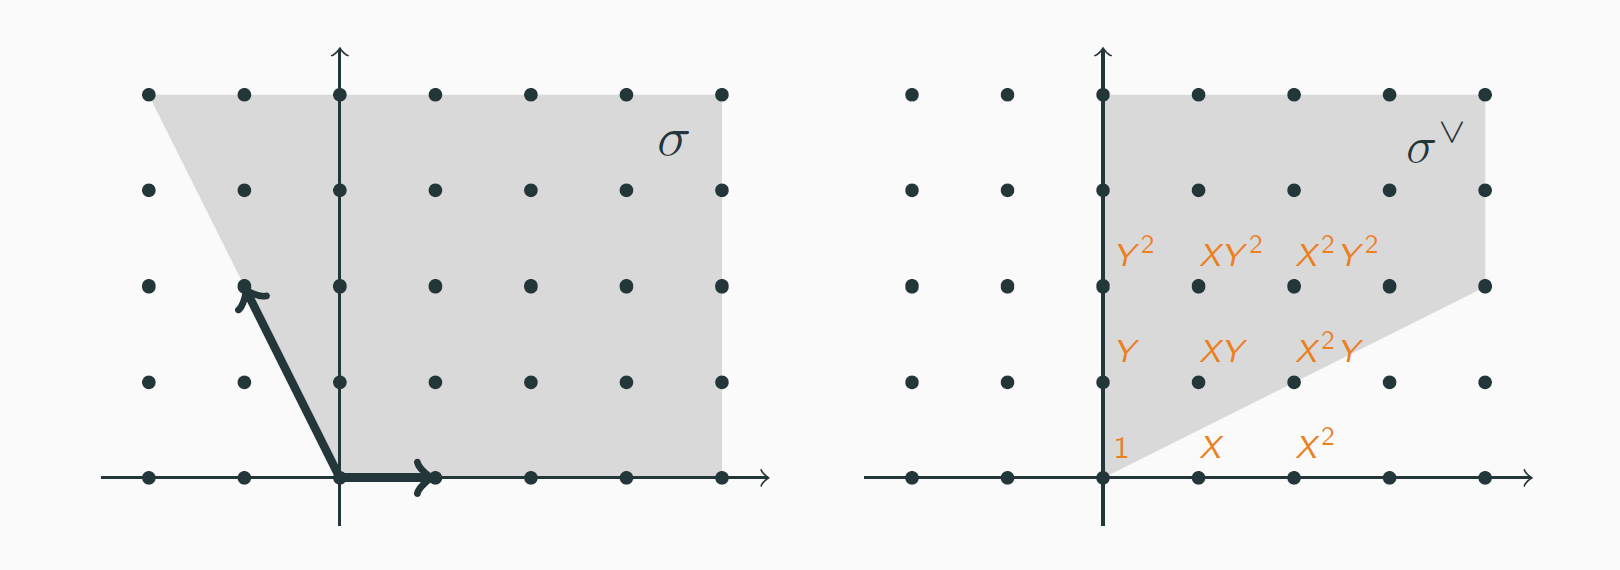
\includegraphics[width=0.8\textwidth]{cone_and_dual_with_monomials}}

We form a ring using the monomials lying in the dual cone:
$$k[1, Y, XY, X^2Y, Y^2, XY^2, \ldots] = k[Y, XY, X^2Y].$$
The toric variety $U_\sigma$ is defined by taking this as its coordinate ring:
$$U_\sigma := \mathrm{Spec}(k[Y, XY, X^2 Y]) = \mathrm{Spec}(k[R, S, T]/(RT - S^2)).$$
\end{frame}

\begin{frame}
\frametitle{Toric varieties, the definition}
The integer points in $\sigma^\vee$ form a \alert{semigroup},
$$S_\sigma := \sigma^\vee \cap (\mathbb{Z}^n)^*.$$
We form the \alert{semigroup algebra} $k[S_\sigma]$.
This has the basis of formula symbols 
$$\{\chi^u : u \in S_\sigma\}$$
with multiplication 
$$\chi^u \chi^{u'} = \chi^{u + u'}.$$
The \alert{toric variety} associated with $\sigma$ is defined as
$$U_\sigma := \mathrm{Spec}(k[S_\sigma]).$$
%``This is our second bridge"
% $\mathbf{V}(XY-ZW)$.
%Do the torus as an example.
\end{frame}

\begin{frame}
\frametitle{The torus in toric varieties}
When $\sigma = \{0\}$, we know $\sigma^\vee = (\mathbb{R}^n)^*$.
The semigroup $S_\sigma$ is
$$S_\sigma = (\mathbb{R}^n)^* \cap (\mathbb{Z}^n)^* = (\mathbb{Z}^n)^*.$$
We see
\begin{align*}
	k[S_\sigma] &= k[\chi^{e_1^*}, \chi^{-e_1^*}, \ldots, \chi^{e_n^*}, \chi^{-e_n^*}] \\
		&= k[X_1, X_1^{-1}, \ldots, X_n, X_n^{-1}]
\end{align*}
Then
$$U_\sigma = \mathrm{Spec}(k[X_1, X_1^{-1}, \ldots, X_n, X_n^{-1}]) = (k^\times)^n$$
is the \alert{algebraic torus}.
\end{frame}

\begin{frame}
\frametitle{Faces}
A \alert{face} of a cone  $\sigma$ is the intersection of $\sigma$ with a hyperplane which contains $\sigma$ in a half-space.

\centerline{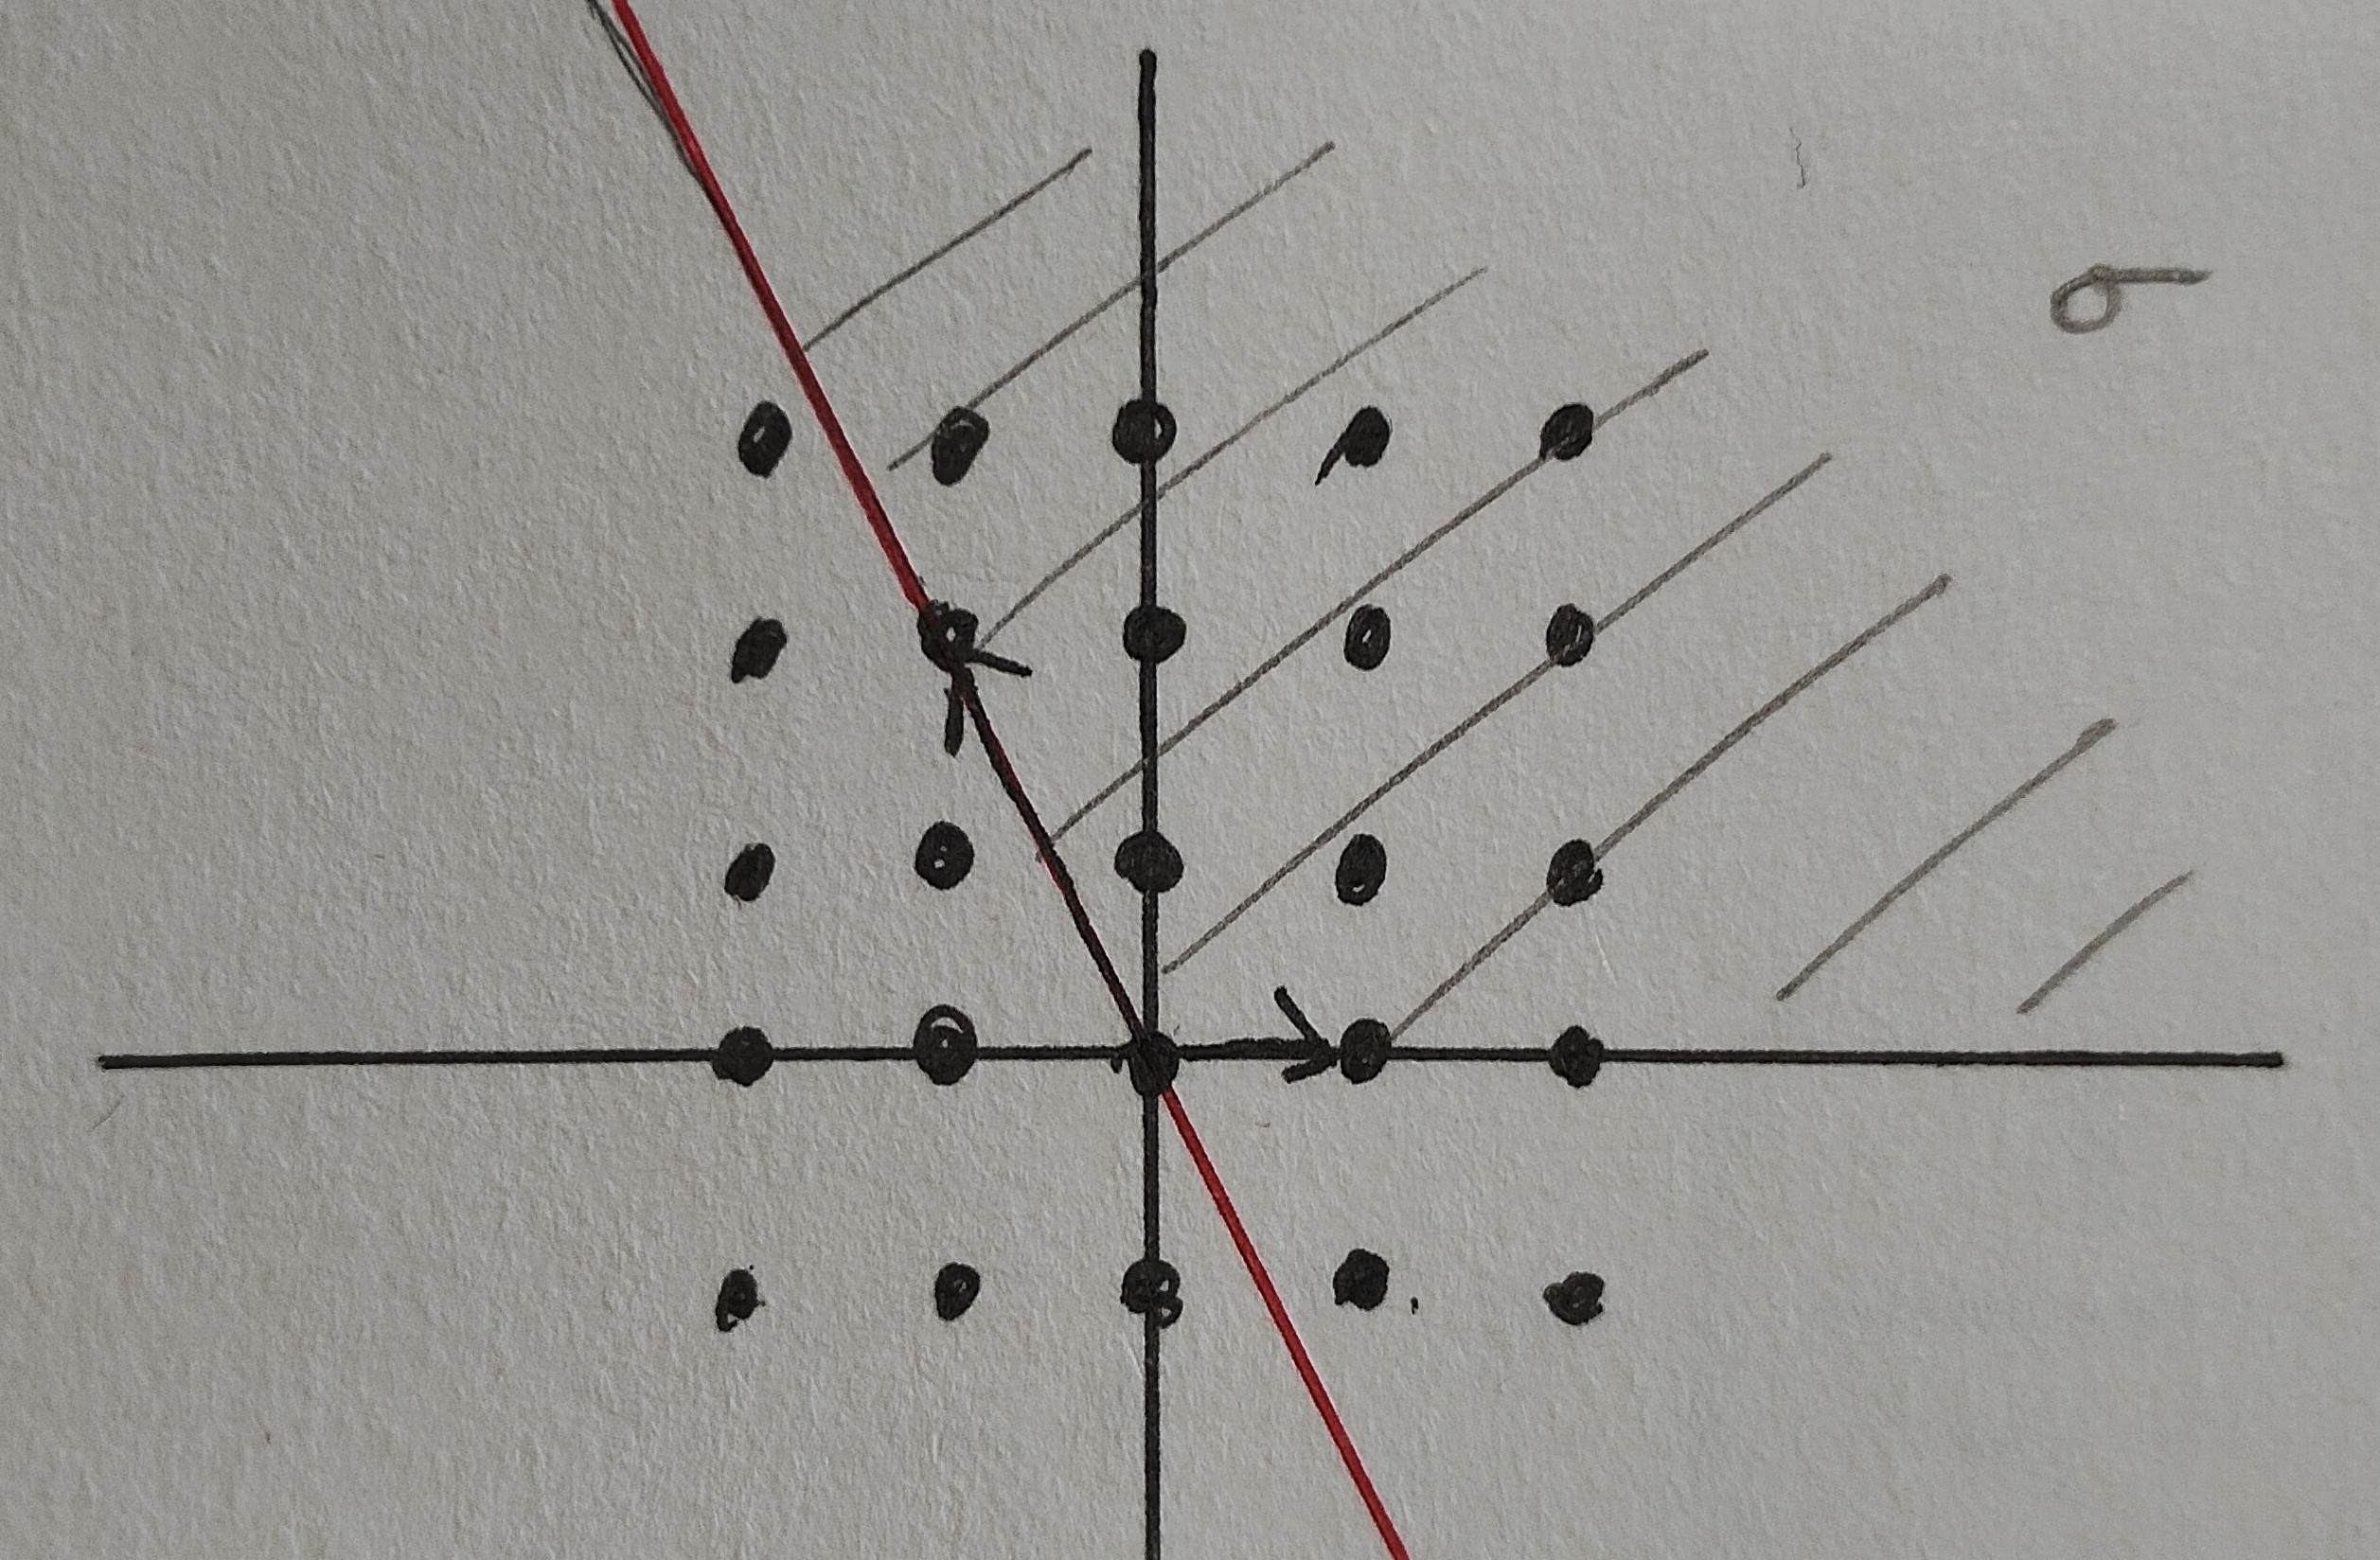
\includegraphics[width=0.4\textwidth]{face}}

If $\tau$ is a face of $\sigma$, then $\tau \subseteq \sigma$ but $\tau^\vee \supseteq \sigma^\vee$ and $S_\tau \supseteq S_\sigma$.
We then have an inclusion 
$$k[S_\sigma] \hookrightarrow k[S_\tau].$$
Corresponding to this, there is a map
$$U_\tau \to U_\sigma.$$
\end{frame}

\begin{frame}
\frametitle{Faces and open subsets}
\begin{theorem}
Let $\tau$ be a face of $\sigma$.
Then the map $U_\tau \to U_\sigma$ embeds $U_\tau$ as a principal open subset of $U_\sigma$.
\end{theorem}

Smaller faces correspond to smaller open subsets.

\centerline{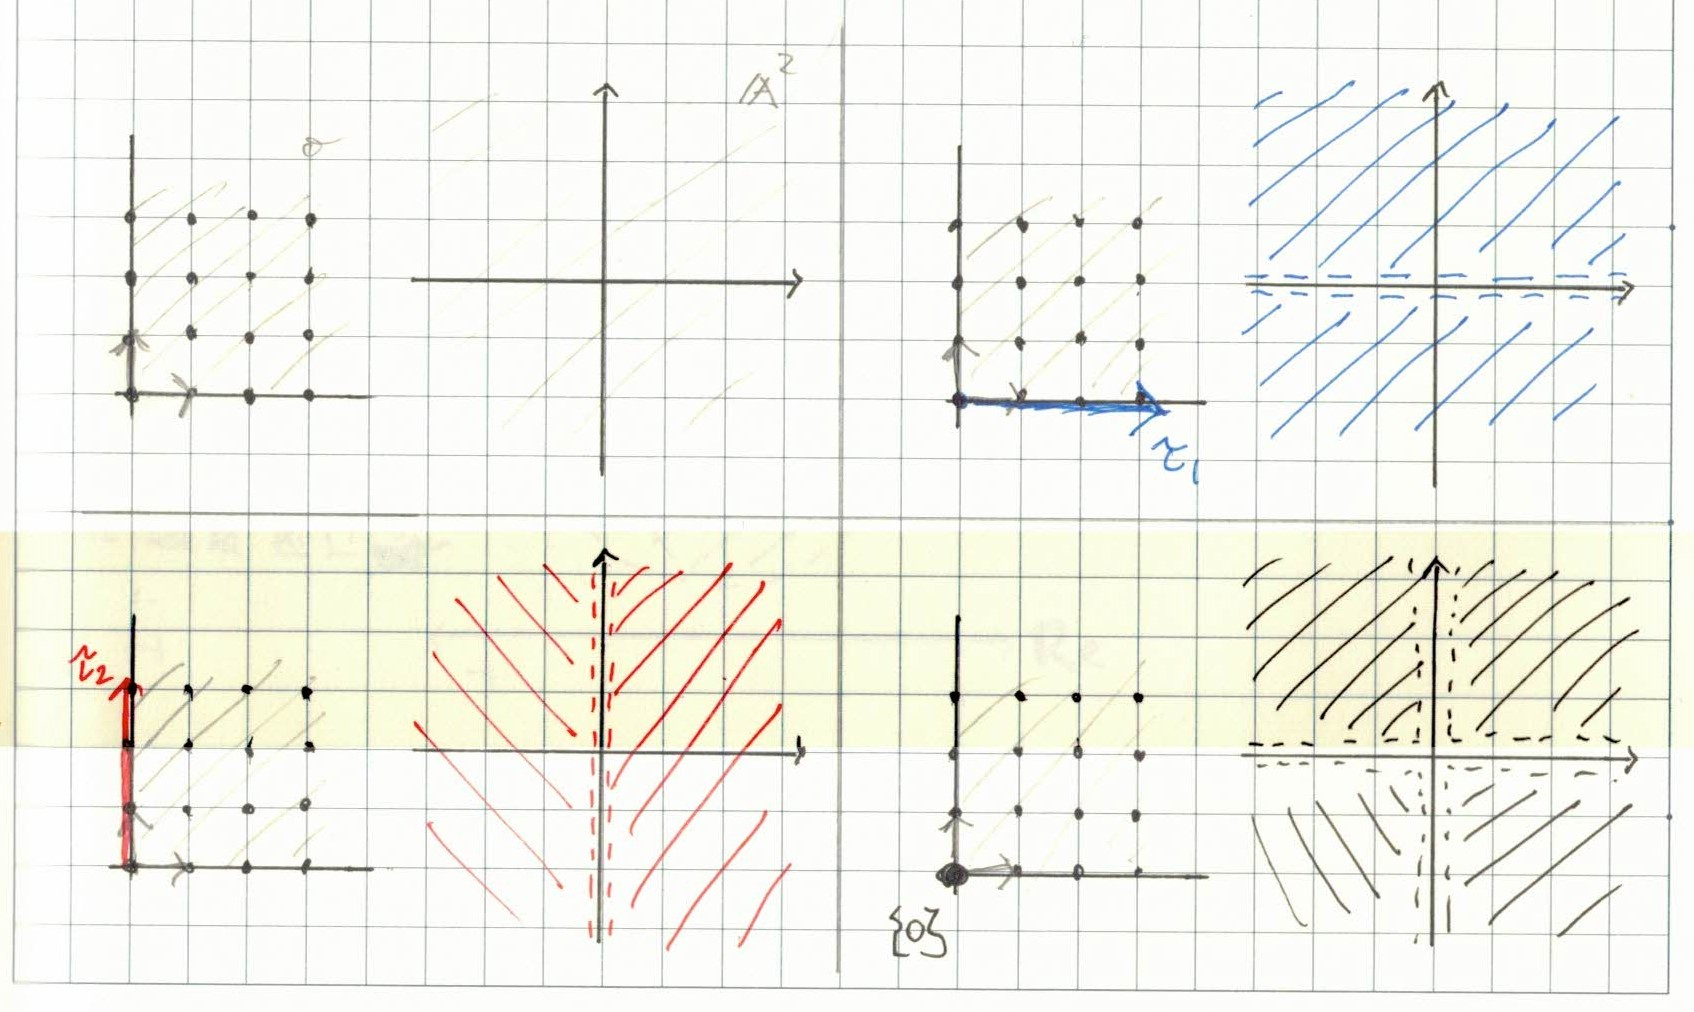
\includegraphics[width=0.8\textwidth]{faces_and_open_sets}}
\end{frame}

\begin{frame}
\frametitle{Singularities of toric varieties}
\begin{theorem}
An toric variety $U_\sigma$ is non-singular if and only if $\sigma$ is generated by a subset of a basis for $\mathbb{Z}^n$.
In this case,
$$U_\sigma \cong k^r \times (k^\times)^{n-r},$$
where $r = \dim(\sigma)$.
\end{theorem}
\end{frame}

\begin{frame}
\frametitle{Cones detect singularities}
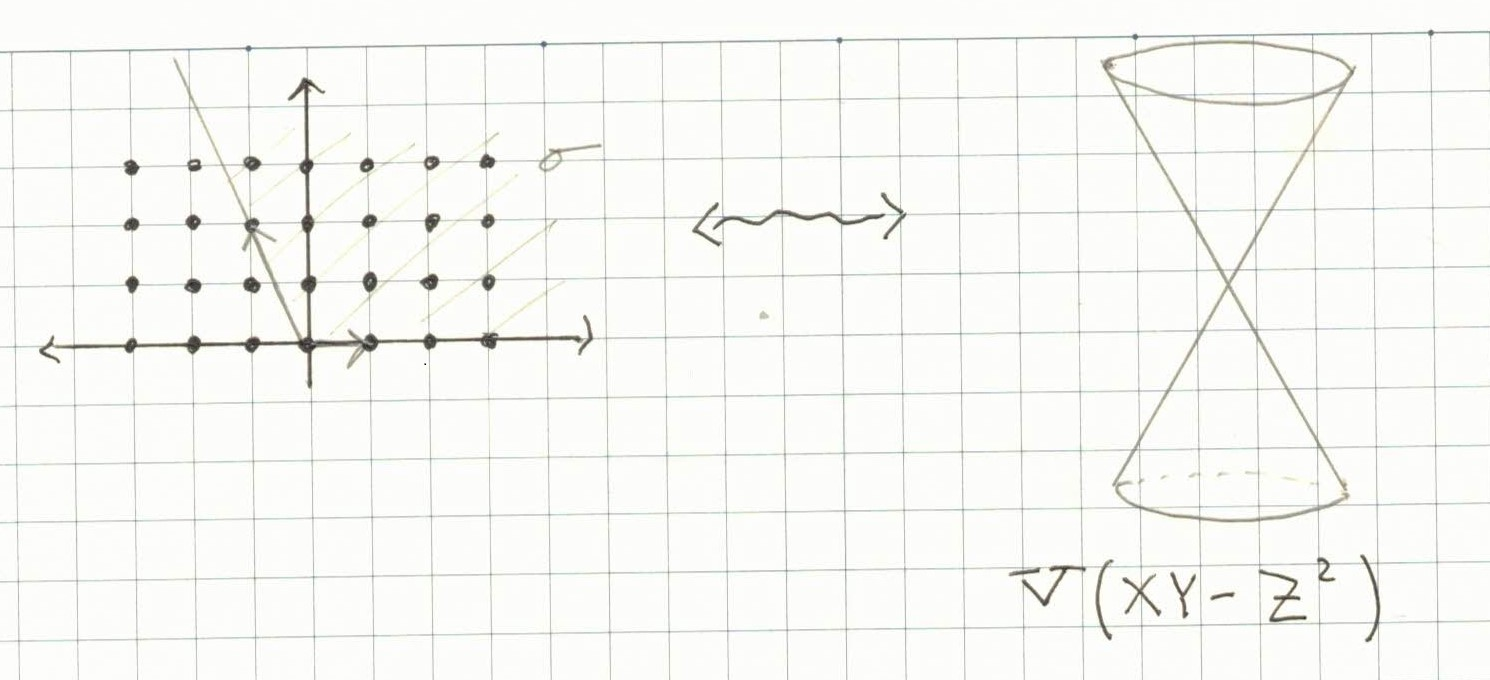
\includegraphics[width=\textwidth]{cone_and_variety}
\end{frame}

\begin{frame}
\frametitle{References}
%\begin{adjustwidth}{-1.7em}{-1.7em}
\begin{enumerate}%[leftmargin=-1cm]
\item[]
David Cox, John Little, and Henry Schenck,
\emph{Toric varieties},
American Mathematical Society, 2011.

\vspace{0.5cm}

\item[]
William Fulton,
\emph{Introduction to toric varieties},
Princeton University Press, 1993.

\vspace{0.5cm}

\item[]
James Milne,
\emph{Algebraic Geometry} (2023),
{ \texttt{www.jmilne.org/math/}}. %\footnotesize

\vspace{0.5cm}

\item[]
Miles Reid,
\emph{Undergraduate algebraic geometry},
Cambridge Univeristy Press, 1988.
\end{enumerate}
%\end{adjustwidth}
\end{frame}
\end{document}